\section{Ethylene pyrolysis in a flow reactor}
The PFR model was used to simulate the pyrolysis of \%0.6 $\mathrm{C_2H_4-N_2}$ in a flow reactor 1.4 m long and 16 mm in diameter. The temperature profile was imposed in the model from the measurement along the reactor centerline by~\citet{mei2019quantitative} for the maximum temperature of 1700 K. The inception models were calibrated using the inception and PAH adsorption scaling factors to match the predicted PSD with measurements at the volumetric flow rates, Q of 8.5, 11 and 12 L/min.

\begin{figure}[H]
	\centering
	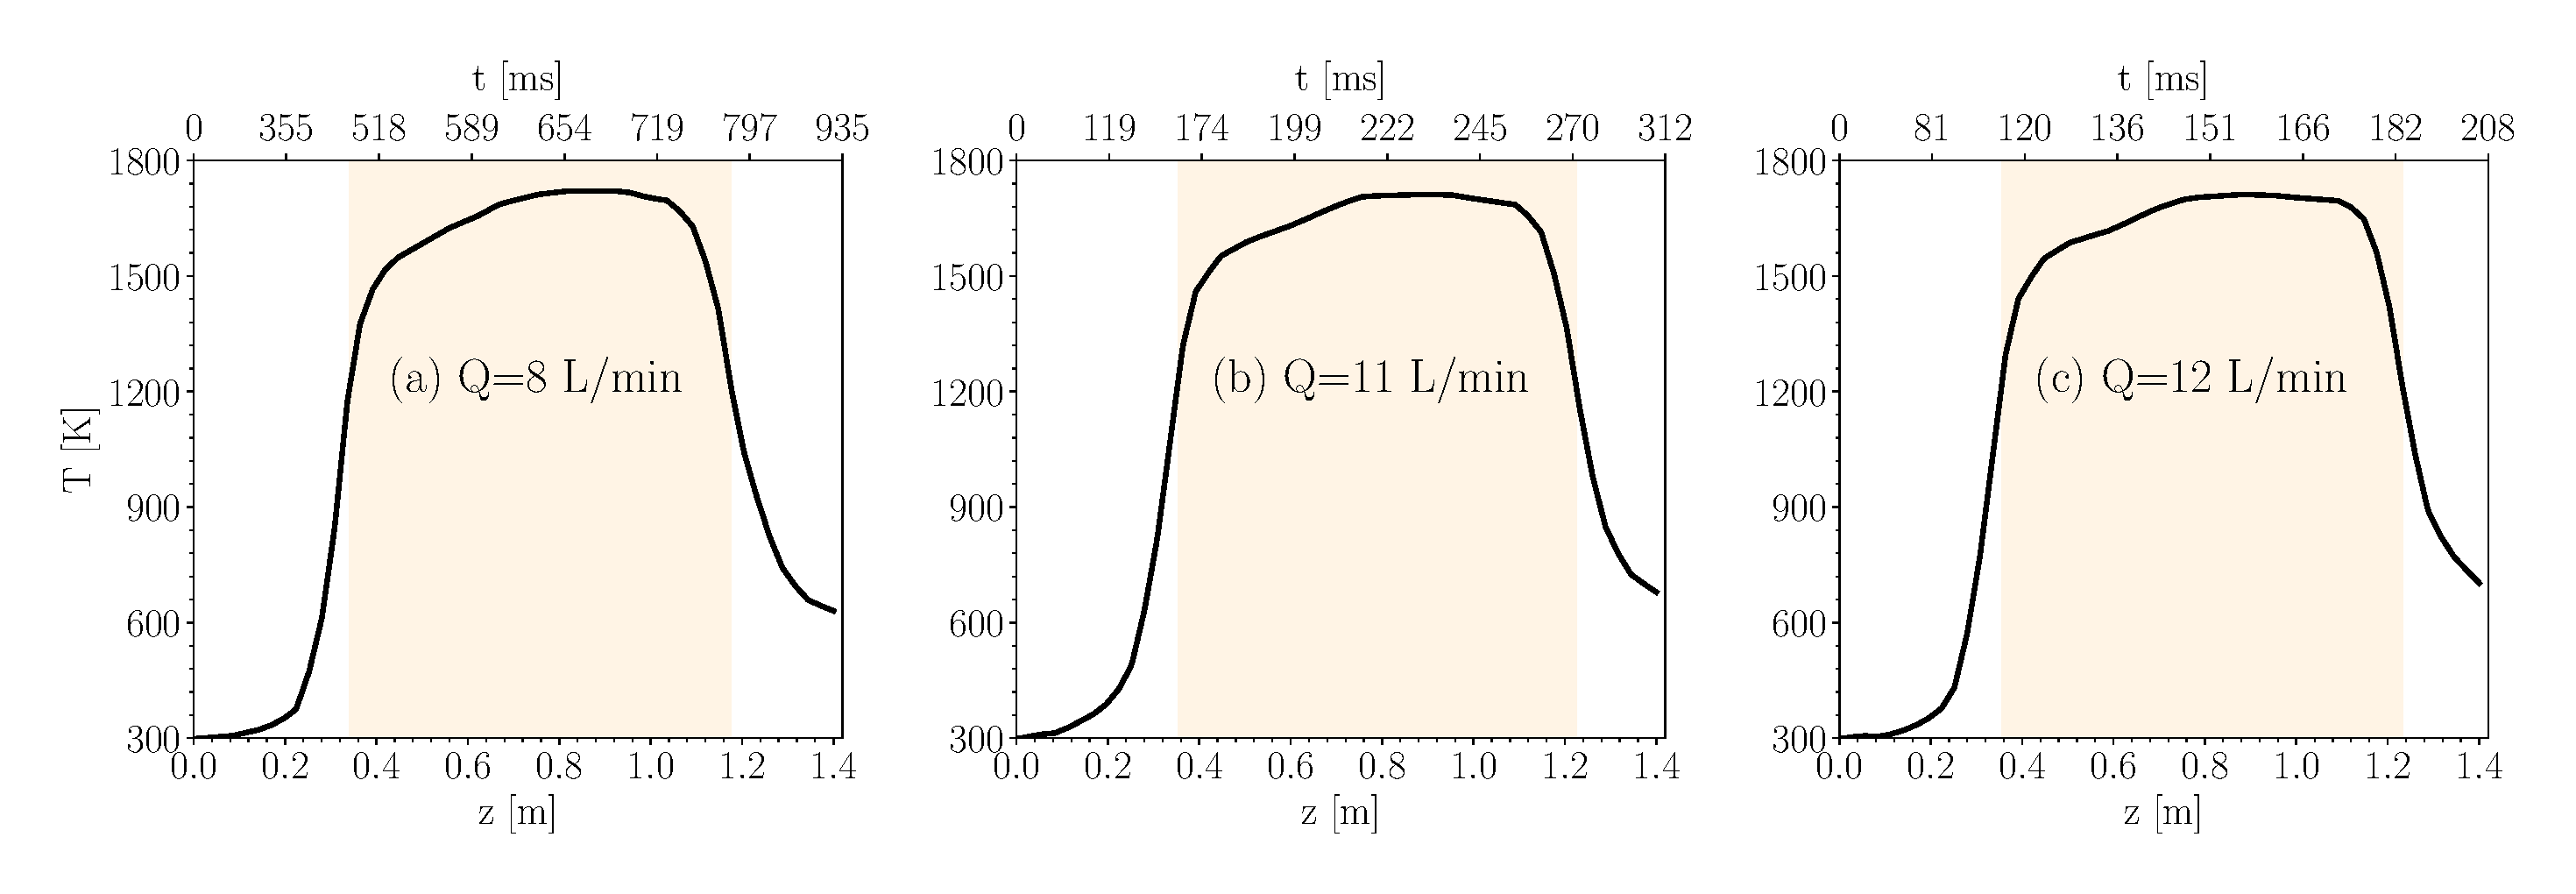
\includegraphics[width=1\textwidth]{Figures/Results/PFR/temperature.pdf}
	\caption{The centerline temperature along the reactor for Q=8 (a), 11 (b), and 12 L/min (c) interpolated from the thermocouple measurements~\citep{mei2019quantitative}. The yellow area represent the region with temperature larger than 1200 K.}
	\label{fig:pfr_temp} 
\end{figure}

\begin{figure}[H]
	\centering
	\begin{tikzpicture}
		\draw (0, 0) node[inner sep=0] 	{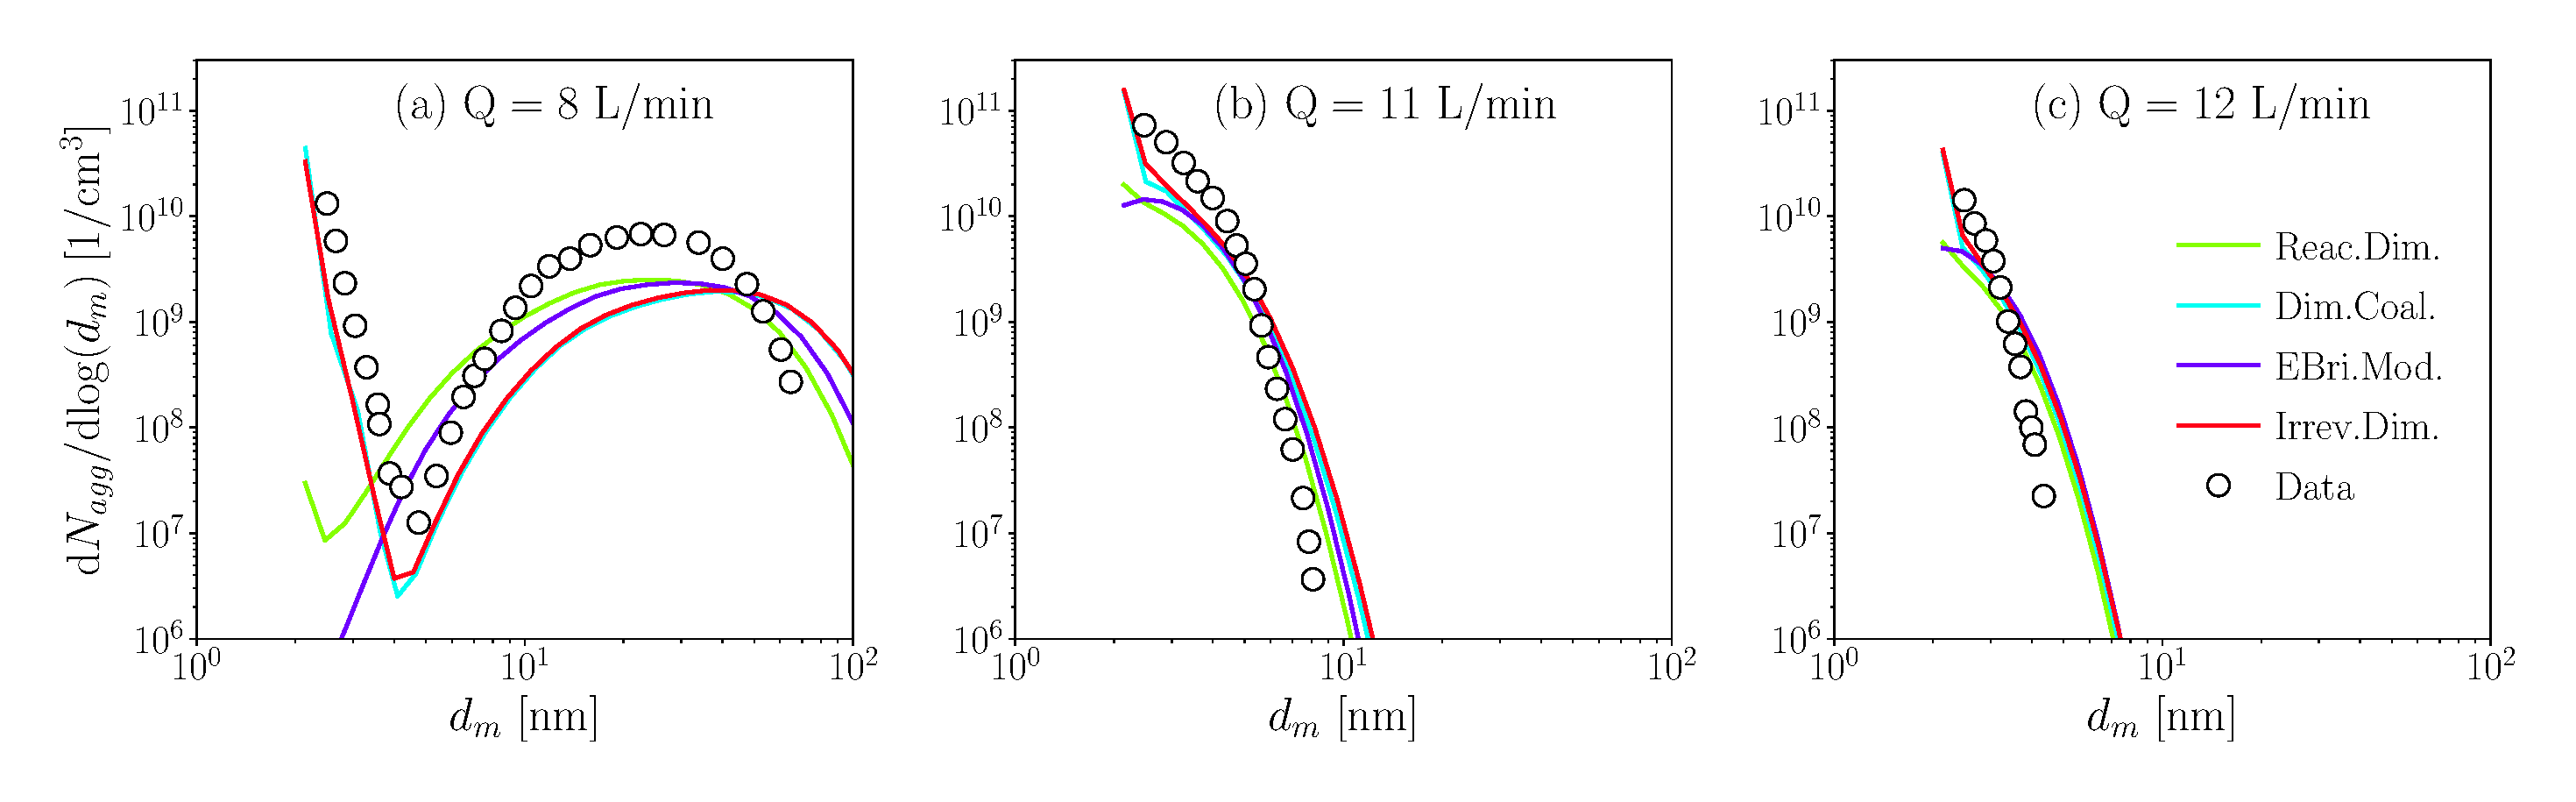
\includegraphics[width=1\textwidth]{Figures/Results/PFR/PSD_diffQ.pdf}};
		\draw (-3.05, -1.1) node {\tiny{\cite{mei2019quantitative}}};
		\draw (1.77, 0.59) node {\tiny{\cite{mei2019quantitative}}};
		\draw (6.63, 0.58) node {\tiny{\cite{mei2019quantitative}}};
	\end{tikzpicture}
	\caption{The particle size distribution at the end of PFR for Q=8.5 (a), 11 (b), and 12 L/min (c) obtained using KAUST mechanism and different inception models calibrated to match the predictions with measurement~\citep{mei2019quantitative}.}
	\label{fig:pfr_psd} 
\end{figure}

\begin{figure}[H]
	\centering
	\begin{tikzpicture}
		\draw (0, 0) node[inner sep=0] 	{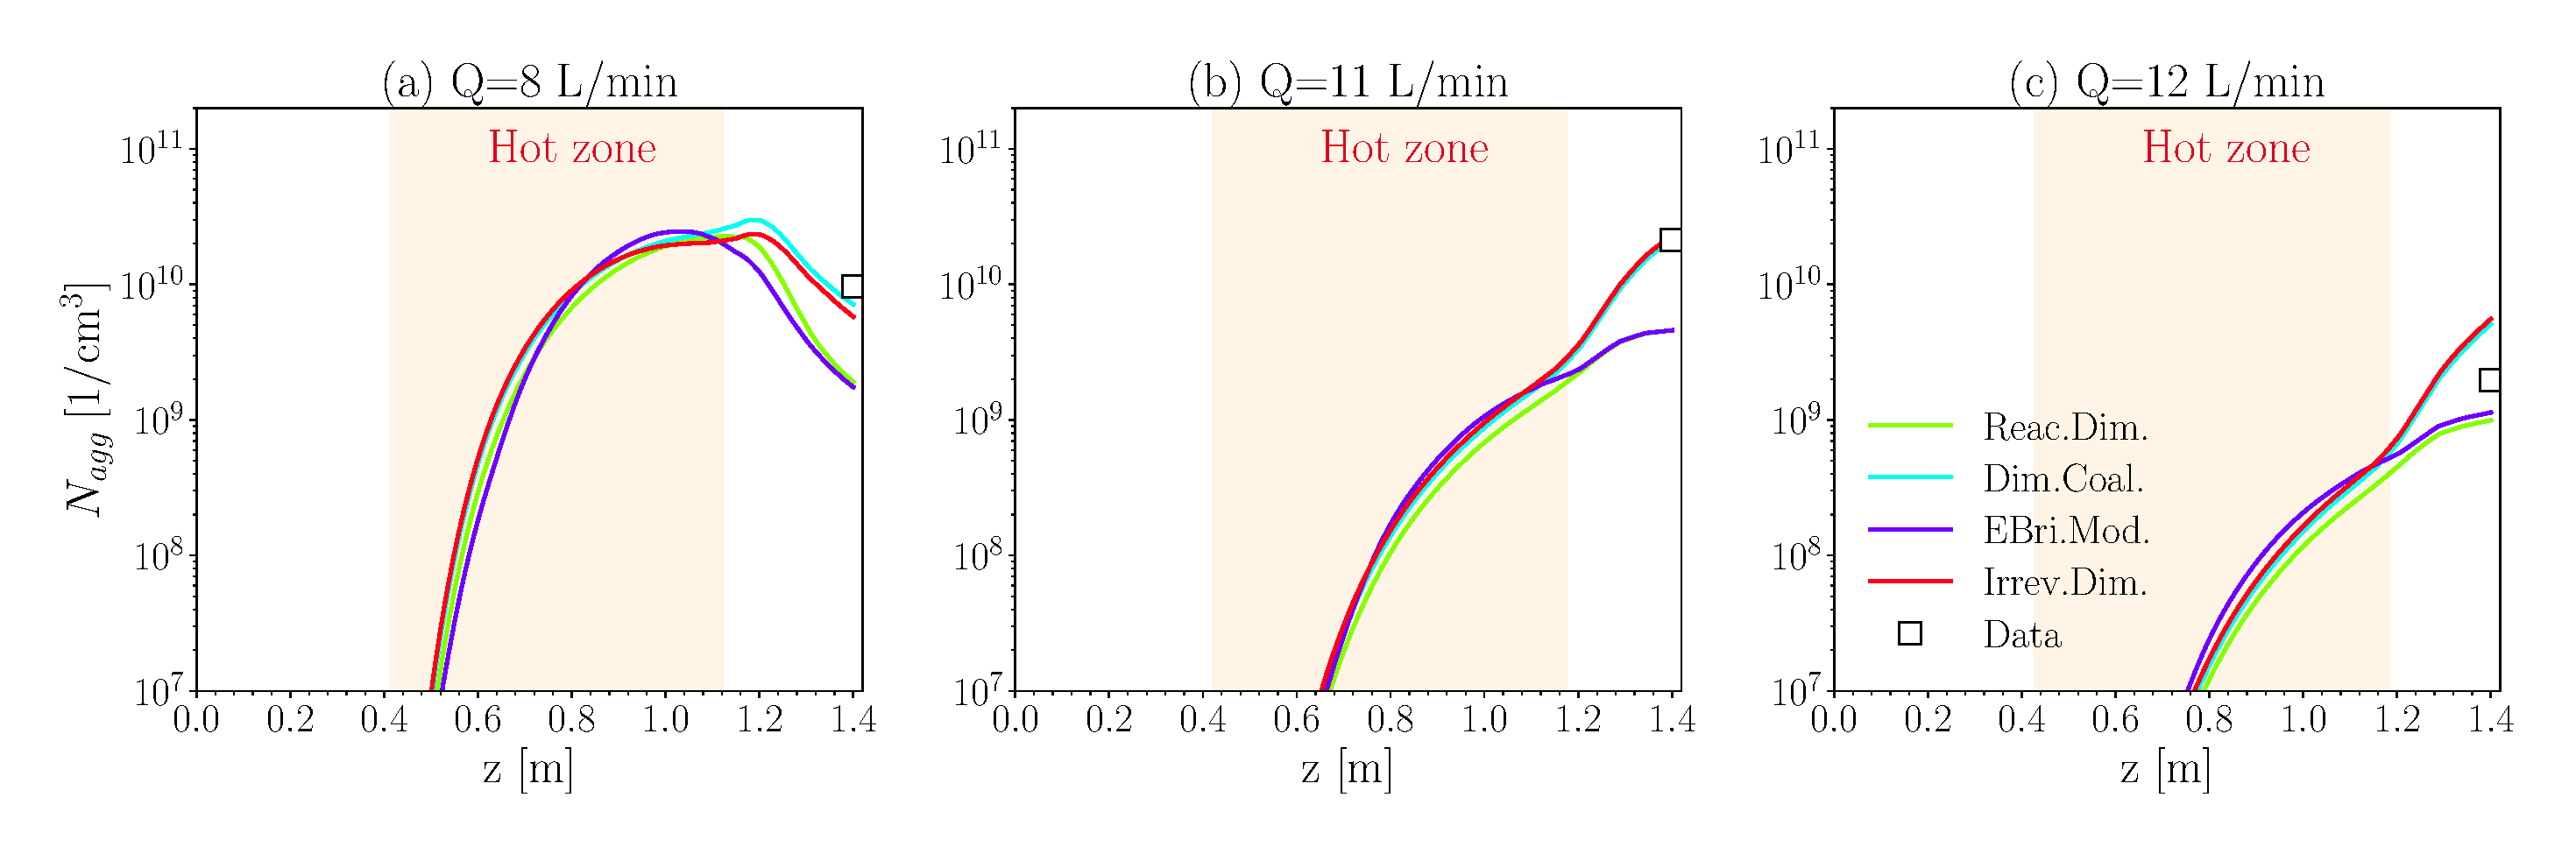
\includegraphics[width=1\textwidth]{Figures/Results/PFR/N_agg.pdf}};
		\draw (-2.9, -1.1) node {\tiny{\cite{mei2019quantitative}}};
	\end{tikzpicture}
	\caption{The total number of agglomerates along the PFR for Q=8.5 (a), 11 (b), and 12 L/min (c) obtained using KAUST mechanism and different inception models compared with data~\citep{mei2019quantitative}.}
	\label{fig:pfr_Nagg} 
\end{figure}

\begin{figure}[H]
	\centering
	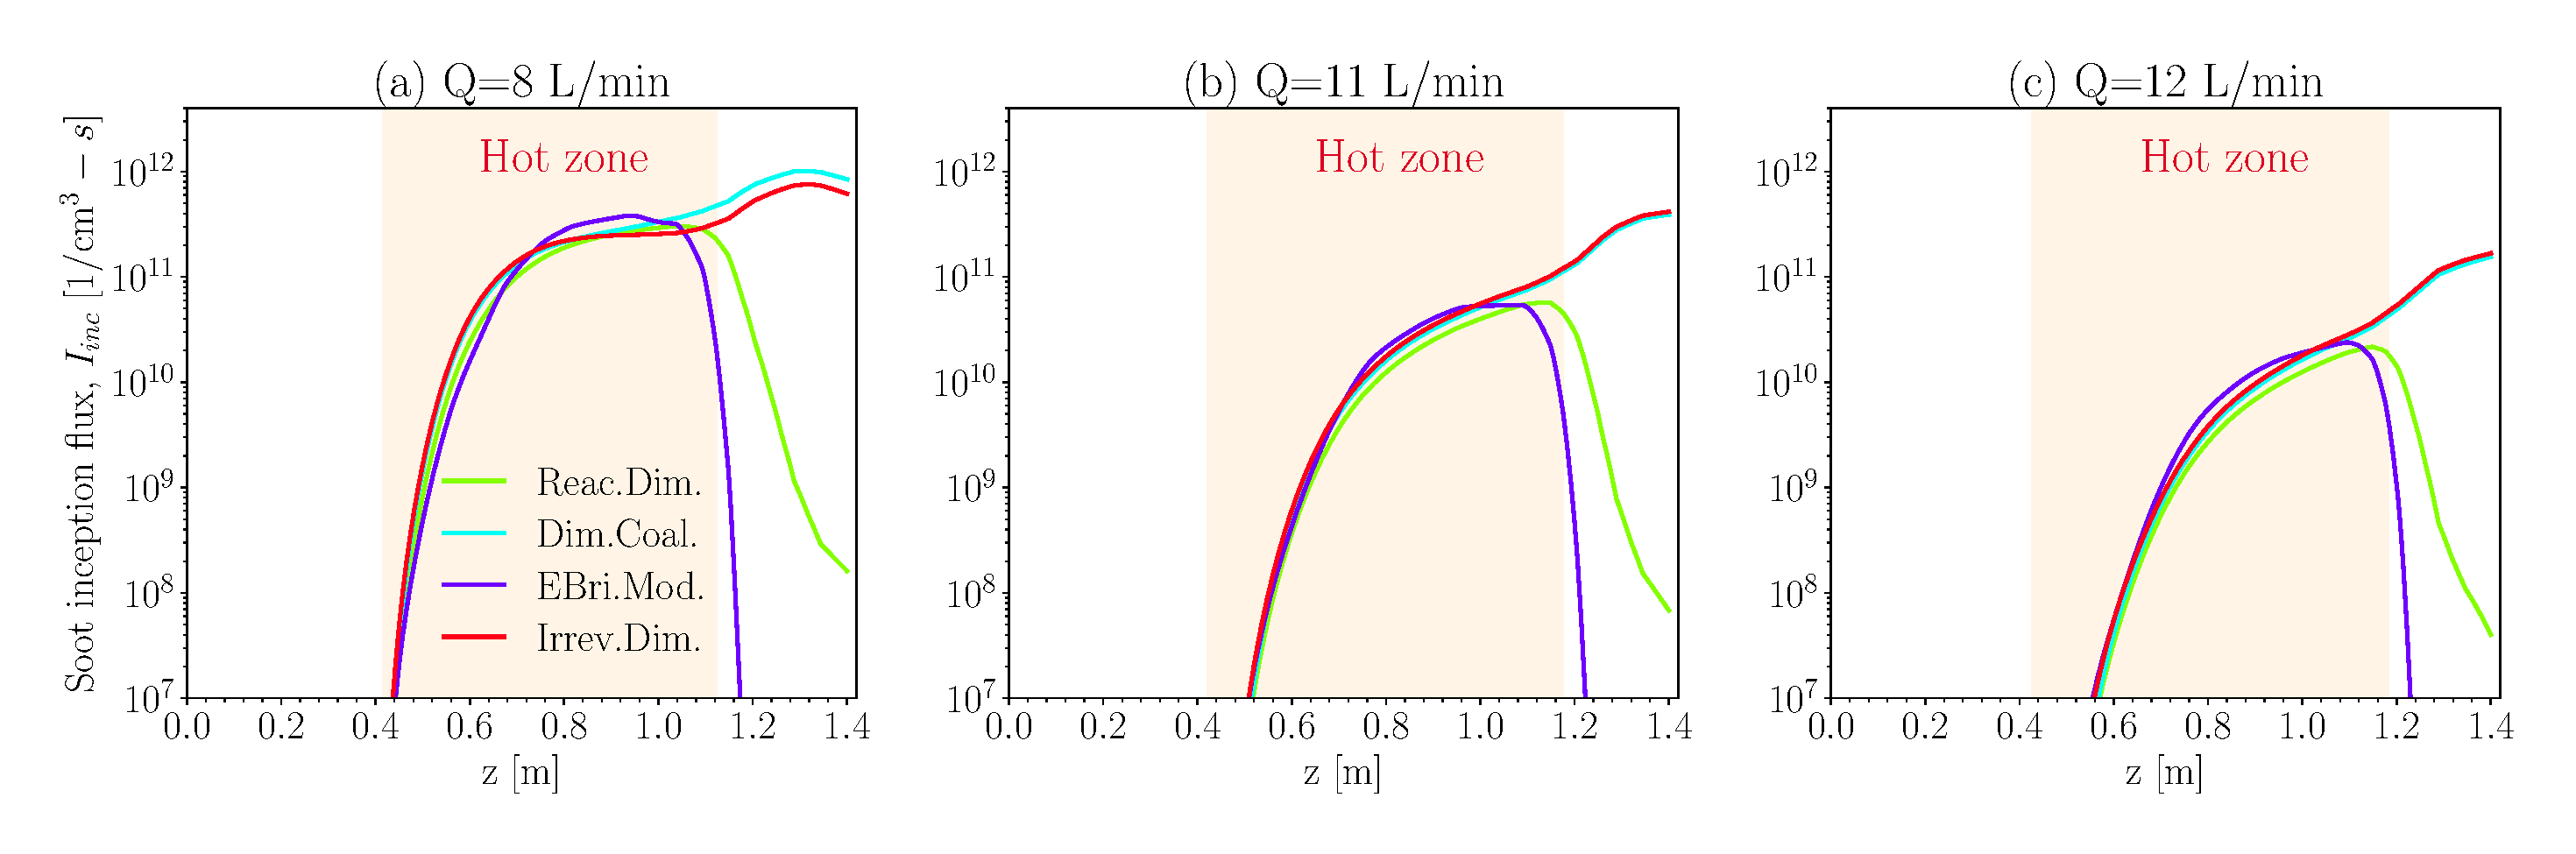
\includegraphics[width=1\textwidth]{Figures/Results/PFR/inception.pdf}
	\caption{The soot inception flux along the PFR for Q=8.5 (a), 11 (b), and 12 L/min (c) obtained using KAUST mechanism and different inception models.}
	\label{fig:pfr_Iinc} 
\end{figure}